\section{Heating and Cooling in HII regions}

In this section we will investigate the equilibrium temperature of heating and cooling rates in an HII region similar to Orion. We will search for these equilibrium temperatures using a root finding algorithm. In this work we have chosen to use only the False Position Method to maintain the convergence guarantee provided by bisection, but increase the convergence speed somewhat. We note that faster convergence is possibly by combining a faster and less accurate in the beginning, with a slower and more accurate algorithm near the root. However this is not implemented here due to time constraints.

% CODE

\subsection{Simple Case}

First we will only consider an HII region with one heating and cooling mechanism. The heating is produced by photoionization given by

\begin{equation}
    \Gamma_{pe} = \alpha_B n_H n_e \psi k_B T_c,\label{eq:gamma_pe}
\end{equation}

and the cooling through radiative recombination:

\begin{equation}
    \Lambda_{rr} = \alpha_Bn_Hn_e\left<E_{rr}\right>,\label{eq:lamda_rr}
\end{equation}

with

\begin{equation}
    \left<E_{rr}\right> = \left[0.684 - 0.0416\ln\left(\frac{T_4}{Z^2}\right)\right]k_BT.
\end{equation}

In these equations, $\alpha_B = 2 \times 10^{-13}$ cm$^3$ s$^{-1}$ is the case B recombination coefficient, $k_B = 1.38\times 10^{-16}$ erg K$^{-1}$ is the Stefan-Boltzmann constant, $\phi = 0.929$ is given, $T_c = 10^4$ K is the stellar temperature, $Z = 0.015$ is the metalicity and $T_4 \equiv \frac{T}{10^4\text{K}}$ is the temperature. Finally, we assume the proton and electron densities to be equal, such that $n_e = n_p$.

The equilibrium temperature $T_eq$ is given by the temperature at which the heating rate is equal to the cooling rate, $\Gamma_{pe} = \Lambda_{rr}$. We can formulate this in terms of a root finding problem by searching for the point where $\Gamma_{pe} - \Lambda_{rr} = 0$. We can work out what this should be by combining equations \ref{eq:gamma_pe} and \ref{eq:lamda_rr} to find that this means the following should hold

\begin{equation}
    \psi T_c - \left[0.684 - 0.0416\ln\left(\frac{T}{10^4\cdot Z^2}\right)\right] \cdot T = 0.
\end{equation}

Note that the densities $n$, $\alpha_B$ and $k$ have all dropped out of this specific equation, even though this does not represent the true difference between heating and cooling rate at other temperatures. This is not important because we are only interested in the temperature at which the above equation is true, where additional scaling factors are important.

We apply our root finding algorithm introduced earlier to this equation with an initial bracket in the range $T = \left[1, 10^7\right]$ K. We aim for a temperature accuracy of $0.1$ K. We present the result in figure \ref{fig:simple_roots}, we can see that we find a root at $T = 3.25 \times 10^4$ K, where the function has a value of $-3.45 \times 10^{-3}$. This is a relatively large value, but the algorithm has converged because it is taking very small steps along the temperature axis.

\begin{figure}
    \centering
    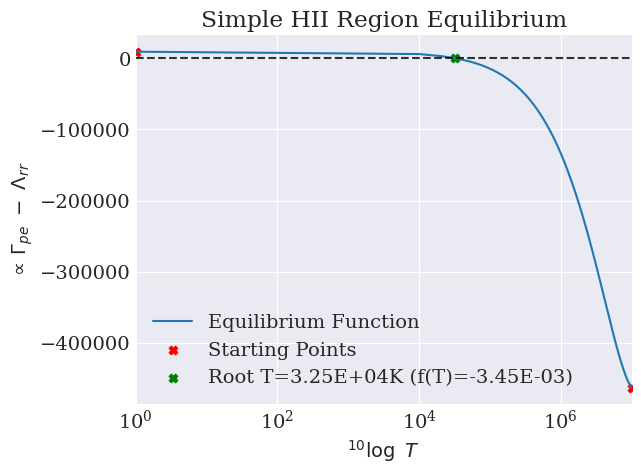
\includegraphics[width=0.8\textwidth]{results/simple_hiiregion_roots.png}
    \caption{}
    \label{fig:simple_roots}
\end{figure}


\subsection{More Complex Case}

In addition to the singular heating and cooling mechanisms we described in the previous section, we will now setup a more realistic scenario and also include cooling through free-free emission ($\Lambda_{ff}$) and heating through cosmic rays ($\Sigma_{cr}$) and magnetohydrodynamic waves ($\Sigma_{MHD}$). These are all individually,given by the following three equations:

\begin{equation}
    \Lambda_{ff} = 0.54 T_4^{0.37}\alpha_Bn_en_hk_BT
\end{equation}
\begin{equation}
    \Gamma_{cr} = An_e\xi_{CR} \\
\end{equation}
\begin{equation}
    \Gamma_{MHD} = 8.9 \times 10^{-26}n_hT_4
\end{equation}

Synonymous to the previous section we can find the equilibrium temperature $T_{eq}$ by finding the temperature for which $\Gamma - \Lambda = 0$ where $\Gamma$ and $\Lambda$ represent the total heating and cooling rate respectively, which are just the sums of each of the individual effects. Working this out, we find that the following equation most hold:

\begin{align}
    \bigg(\psi T_c - \left[0.684 - 0.0416\left(\frac{T}{10^4\cdot Z^2}\right)\right] \cdot T &- 0.54 \left(\frac{T}{10^4}\right) T \bigg)\cdot k_Bn_H\alpha_B\nonumber \\
    ... &+ A\xi + 8.9 \times 10^{-26}n_H\frac{T}{10^4} = 0\label{eq:equi2}
\end{align}
